\subsubsection{Overview}
The Depth First Search (DFS) is the most fundamental search algorithm used to explore nodes and edges of a graph. It runs with a time complexity of $O(V+E)$ and is often used as a building block in other algorithms.\\

By itself the DFS is not all that useful, but when augmented to perform other tasks such as count connected components, determine connectivity, or find bridges / articulation points then DFS really shines.


\subsubsection{Basic DFS}
As the name suggest, a DFS plunges depth first into a graph without regard for which edge it takes next until it cannot go any further at which point it backtracks and continues.\\

Lets give an example using the next graph

\begin{figure}[H]
\begin{center}
    \begin{tikzpicture}[scale=0.2]
    \tikzstyle{every node}+=[inner sep=0pt]
    \draw [black] (5.4,-28.9) circle (3);
    \draw (5.4,-28.9) node {$0$};
    \draw [black] (16.3,-24) circle (3);
    \draw (16.3,-24) node {$1$};
    \draw [black] (16.3,-34.3) circle (3);
    \draw (16.3,-34.3) node {$9$};
    \draw [black] (25.6,-28.9) circle (3);
    \draw (25.6,-28.9) node {$8$};
    \draw [black] (36.4,-38.2) circle (3);
    \draw (36.4,-38.2) node {$7$};
    \draw [black] (28.4,-49.8) circle (3);
    \draw (28.4,-49.8) node {$10$};
    \draw [black] (43.2,-49.8) circle (3);
    \draw (43.2,-49.8) node {$11$};
    \draw [black] (52.8,-38.2) circle (3);
    \draw (52.8,-38.2) node {$6$};
    \draw [black] (59.7,-26.9) circle (3);
    \draw (59.7,-26.9) node {$5$};
    \draw [black] (45.4,-25.2) circle (3);
    \draw (45.4,-25.2) node {$3$};
    \draw [black] (56.1,-10.2) circle (3);
    \draw (56.1,-10.2) node {$4$};
    \draw [black] (40.2,-9.1) circle (3);
    \draw (40.2,-9.1) node {$2$};
    \draw [black] (26.6,-13.1) circle (3);
    \draw (26.6,-13.1) node {$12$};
    \draw [black] (8.14,-27.67) -- (13.56,-25.23);
    \draw [black] (8.09,-30.23) -- (13.61,-32.97);
    \draw [black] (18.95,-25.4) -- (22.95,-27.5);
    \draw [black] (18.89,-32.79) -- (23.01,-30.41);
    \draw [black] (27.87,-30.86) -- (34.13,-36.24);
    \draw [black] (34.7,-40.67) -- (30.1,-47.33);
    \draw [black] (37.92,-40.79) -- (41.68,-47.21);
    \draw [black] (31.4,-49.8) -- (40.2,-49.8);
    \draw [black] (39.4,-38.2) -- (49.8,-38.2);
    \draw [black] (38.11,-35.73) -- (43.69,-27.67);
    \draw [black] (48.38,-25.55) -- (56.72,-26.55);
    \draw [black] (54.36,-35.64) -- (58.14,-29.46);
    \draw [black] (47.14,-22.76) -- (54.36,-12.64);
    \draw [black] (44.48,-22.35) -- (41.12,-11.95);
    \end{tikzpicture}
    \end{center}
\end{figure}

The DFS starts in the node 0


\begin{figure}[H]
\begin{center}
    \begin{tikzpicture}[scale=0.2]
    \tikzstyle{every node}+=[inner sep=0pt]
    \draw [black] (5.4,-28.9) circle (3);
    \draw (5.4,-28.9) node {$0$};
    \draw [black] (5.4,-28.9) circle (2.4);
    \draw [black] (16.3,-24) circle (3);
    \draw (16.3,-24) node {$1$};
    \draw [black] (16.3,-34.3) circle (3);
    \draw (16.3,-34.3) node {$9$};
    \draw [black] (25.6,-28.9) circle (3);
    \draw (25.6,-28.9) node {$8$};
    \draw [black] (36.4,-38.2) circle (3);
    \draw (36.4,-38.2) node {$7$};
    \draw [black] (28.4,-49.8) circle (3);
    \draw (28.4,-49.8) node {$10$};
    \draw [black] (43.2,-49.8) circle (3);
    \draw (43.2,-49.8) node {$11$};
    \draw [black] (52.8,-38.2) circle (3);
    \draw (52.8,-38.2) node {$6$};
    \draw [black] (59.7,-26.9) circle (3);
    \draw (59.7,-26.9) node {$5$};
    \draw [black] (45.4,-25.2) circle (3);
    \draw (45.4,-25.2) node {$3$};
    \draw [black] (56.1,-10.2) circle (3);
    \draw (56.1,-10.2) node {$4$};
    \draw [black] (40.2,-9.1) circle (3);
    \draw (40.2,-9.1) node {$2$};
    \draw [black] (26.6,-13.1) circle (3);
    \draw (26.6,-13.1) node {$12$};
    \draw [black] (8.14,-27.67) -- (13.56,-25.23);
    \draw [black] (8.09,-30.23) -- (13.61,-32.97);
    \draw [black] (18.95,-25.4) -- (22.95,-27.5);
    \draw [black] (18.89,-32.79) -- (23.01,-30.41);
    \draw [black] (27.87,-30.86) -- (34.13,-36.24);
    \draw [black] (34.7,-40.67) -- (30.1,-47.33);
    \draw [black] (37.92,-40.79) -- (41.68,-47.21);
    \draw [black] (31.4,-49.8) -- (40.2,-49.8);
    \draw [black] (39.4,-38.2) -- (49.8,-38.2);
    \draw [black] (38.11,-35.73) -- (43.69,-27.67);
    \draw [black] (48.38,-25.55) -- (56.72,-26.55);
    \draw [black] (54.36,-35.64) -- (58.14,-29.46);
    \draw [black] (47.14,-22.76) -- (54.36,-12.64);
    \draw [black] (44.48,-22.35) -- (41.12,-11.95);
    \end{tikzpicture}
\end{center}
\end{figure}

Then the DFS moves through an edge and goes to another node, for example node 9, then node 8, then node 7, then node 10, then node 11 and again node 7


\begin{figure}[H]
\begin{center}
    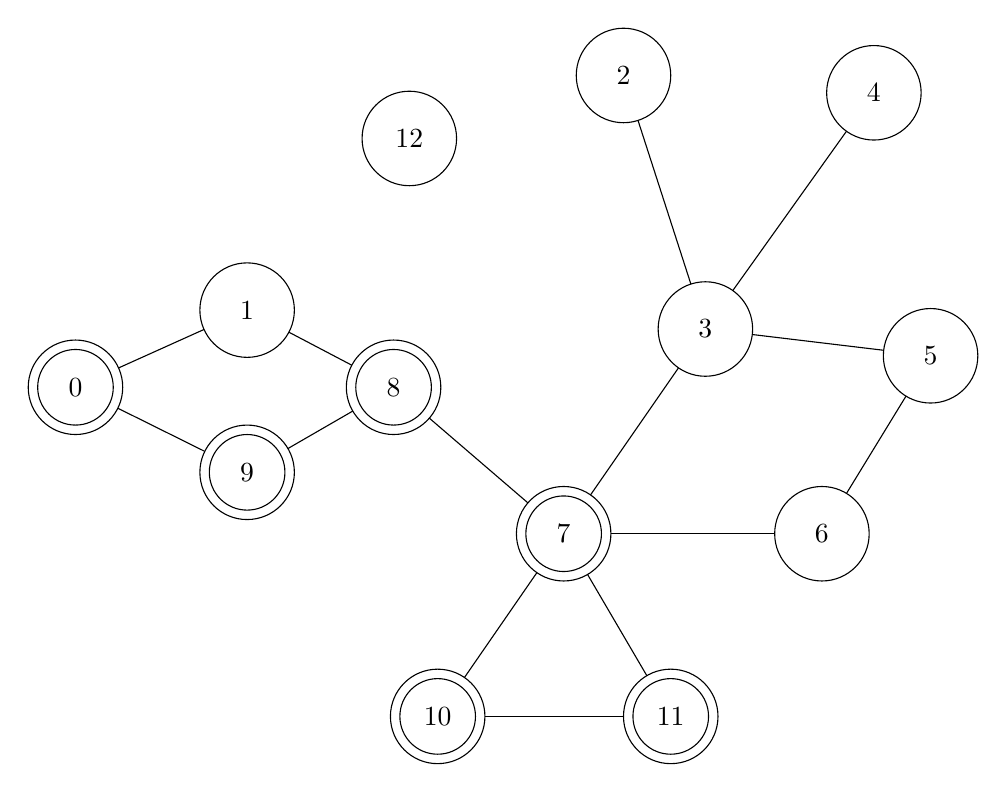
\begin{tikzpicture}[scale=0.2]
    \tikzstyle{every node}+=[inner sep=0pt]
    \draw [black] (5.4,-28.9) circle (3);
    \draw (5.4,-28.9) node {$0$};
    \draw [black] (5.4,-28.9) circle (2.4);
    \draw [black] (16.3,-24) circle (3);
    \draw (16.3,-24) node {$1$};
    \draw [black] (16.3,-34.3) circle (3);
    \draw (16.3,-34.3) node {$9$};
    \draw [black] (16.3,-34.3) circle (2.4);
    \draw [black] (25.6,-28.9) circle (3);
    \draw (25.6,-28.9) node {$8$};
    \draw [black] (25.6,-28.9) circle (2.4);
    \draw [black] (36.4,-38.2) circle (3);
    \draw (36.4,-38.2) node {$7$};
    \draw [black] (36.4,-38.2) circle (2.4);
    \draw [black] (28.4,-49.8) circle (3);
    \draw (28.4,-49.8) node {$10$};
    \draw [black] (28.4,-49.8) circle (2.4);
    \draw [black] (43.2,-49.8) circle (3);
    \draw (43.2,-49.8) node {$11$};
    \draw [black] (43.2,-49.8) circle (2.4);
    \draw [black] (52.8,-38.2) circle (3);
    \draw (52.8,-38.2) node {$6$};
    \draw [black] (59.7,-26.9) circle (3);
    \draw (59.7,-26.9) node {$5$};
    \draw [black] (45.4,-25.2) circle (3);
    \draw (45.4,-25.2) node {$3$};
    \draw [black] (56.1,-10.2) circle (3);
    \draw (56.1,-10.2) node {$4$};
    \draw [black] (40.2,-9.1) circle (3);
    \draw (40.2,-9.1) node {$2$};
    \draw [black] (26.6,-13.1) circle (3);
    \draw (26.6,-13.1) node {$12$};
    \draw [black] (8.14,-27.67) -- (13.56,-25.23);
    \draw [black] (8.09,-30.23) -- (13.61,-32.97);
    \draw [black] (18.95,-25.4) -- (22.95,-27.5);
    \draw [black] (18.89,-32.79) -- (23.01,-30.41);
    \draw [black] (27.87,-30.86) -- (34.13,-36.24);
    \draw [black] (34.7,-40.67) -- (30.1,-47.33);
    \draw [black] (37.92,-40.79) -- (41.68,-47.21);
    \draw [black] (31.4,-49.8) -- (40.2,-49.8);
    \draw [black] (39.4,-38.2) -- (49.8,-38.2);
    \draw [black] (38.11,-35.73) -- (43.69,-27.67);
    \draw [black] (48.38,-25.55) -- (56.72,-26.55);
    \draw [black] (54.36,-35.64) -- (58.14,-29.46);
    \draw [black] (47.14,-22.76) -- (54.36,-12.64);
    \draw [black] (44.48,-22.35) -- (41.12,-11.95);
    \end{tikzpicture}
\end{center}
\end{figure}

We already visited the node 7, so we need to return using backtracking an visit the rest of neighbours of node 7 so we continue doing the DFS but in another direction and we put a mark in the nodes that we already visited but are not valid.

\begin{figure}[H]
\begin{center}
    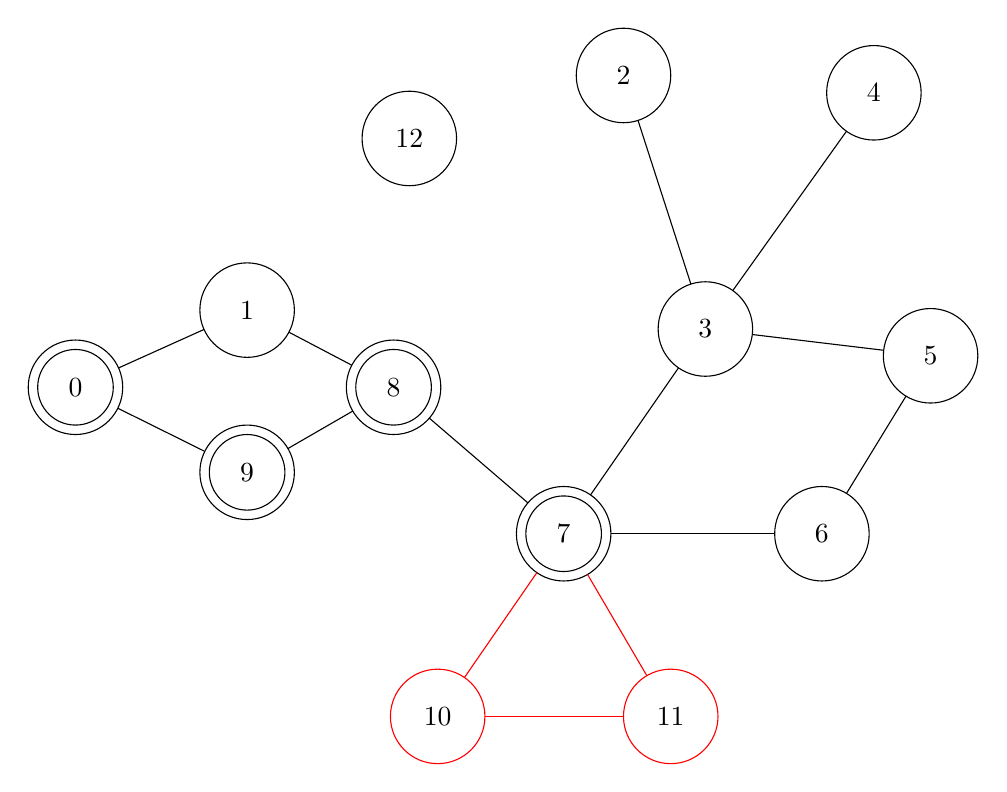
\begin{tikzpicture}[scale=0.2]
    \tikzstyle{every node}+=[inner sep=0pt]
    \draw [black] (5.4,-28.9) circle (3);
    \draw (5.4,-28.9) node {$0$};
    \draw [black] (5.4,-28.9) circle (2.4);
    \draw [black] (16.3,-24) circle (3);
    \draw (16.3,-24) node {$1$};
    \draw [black] (16.3,-34.3) circle (3);
    \draw (16.3,-34.3) node {$9$};
    \draw [black] (16.3,-34.3) circle (2.4);
    \draw [black] (25.6,-28.9) circle (3);
    \draw (25.6,-28.9) node {$8$};
    \draw [black] (25.6,-28.9) circle (2.4);
    \draw [black] (36.4,-38.2) circle (3);
    \draw (36.4,-38.2) node {$7$};
    \draw [black] (36.4,-38.2) circle (2.4);
    \draw [red] (28.4,-49.8) circle (3);
    \draw (28.4,-49.8) node {$10$};
    \draw [red] (43.2,-49.8) circle (3);
    \draw (43.2,-49.8) node {$11$};
    \draw [black] (52.8,-38.2) circle (3);
    \draw (52.8,-38.2) node {$6$};
    \draw [black] (59.7,-26.9) circle (3);
    \draw (59.7,-26.9) node {$5$};
    \draw [black] (45.4,-25.2) circle (3);
    \draw (45.4,-25.2) node {$3$};
    \draw [black] (56.1,-10.2) circle (3);
    \draw (56.1,-10.2) node {$4$};
    \draw [black] (40.2,-9.1) circle (3);
    \draw (40.2,-9.1) node {$2$};
    \draw [black] (26.6,-13.1) circle (3);
    \draw (26.6,-13.1) node {$12$};
    \draw [black] (8.14,-27.67) -- (13.56,-25.23);
    \draw [black] (8.09,-30.23) -- (13.61,-32.97);
    \draw [black] (18.95,-25.4) -- (22.95,-27.5);
    \draw [black] (18.89,-32.79) -- (23.01,-30.41);
    \draw [black] (27.87,-30.86) -- (34.13,-36.24);
    \draw [red] (34.7,-40.67) -- (30.1,-47.33);
    \draw [red] (37.92,-40.79) -- (41.68,-47.21);
    \draw [red] (31.4,-49.8) -- (40.2,-49.8);
    \draw [black] (39.4,-38.2) -- (49.8,-38.2);
    \draw [black] (38.11,-35.73) -- (43.69,-27.67);
    \draw [black] (48.38,-25.55) -- (56.72,-26.55);
    \draw [black] (54.36,-35.64) -- (58.14,-29.46);
    \draw [black] (47.14,-22.76) -- (54.36,-12.64);
    \draw [black] (44.48,-22.35) -- (41.12,-11.95);
    \end{tikzpicture}
\end{center}
\end{figure}

Now we move to the node 3 and then to the node 2 so we need to make backtracking again and continue with our DFS

\begin{figure}[H]
\begin{center}
    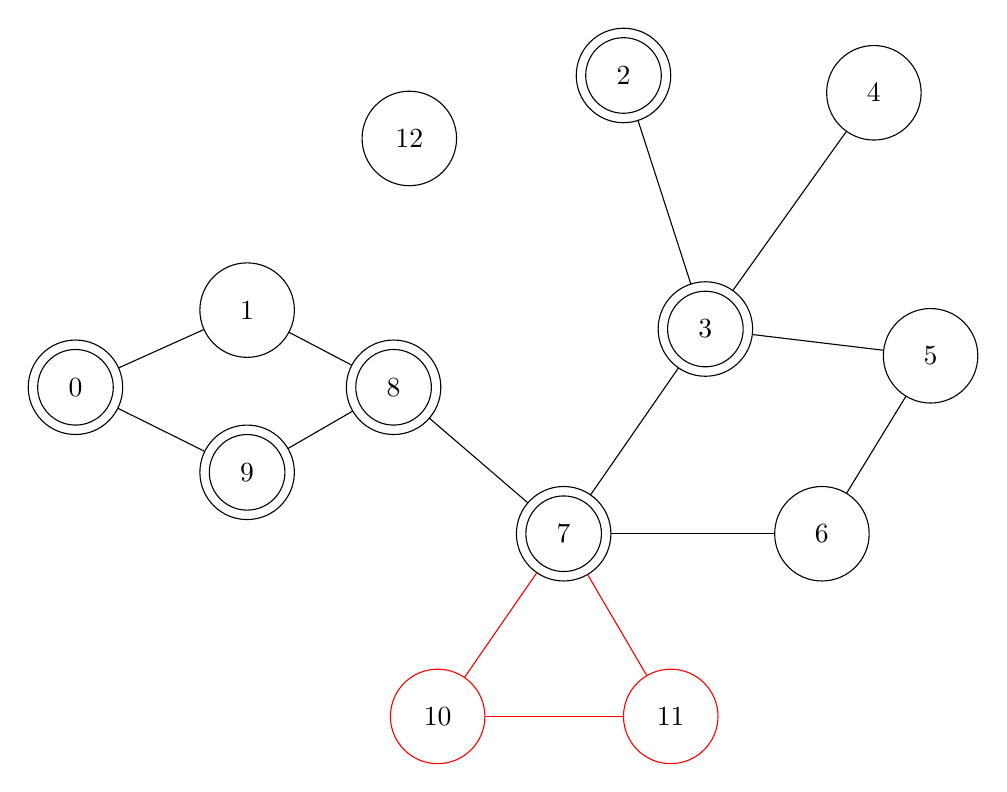
\begin{tikzpicture}[scale=0.2]
    \tikzstyle{every node}+=[inner sep=0pt]
    \draw [black] (5.4,-28.9) circle (3);
    \draw (5.4,-28.9) node {$0$};
    \draw [black] (5.4,-28.9) circle (2.4);
    \draw [black] (16.3,-24) circle (3);
    \draw (16.3,-24) node {$1$};
    \draw [black] (16.3,-34.3) circle (3);
    \draw (16.3,-34.3) node {$9$};
    \draw [black] (16.3,-34.3) circle (2.4);
    \draw [black] (25.6,-28.9) circle (3);
    \draw (25.6,-28.9) node {$8$};
    \draw [black] (25.6,-28.9) circle (2.4);
    \draw [black] (36.4,-38.2) circle (3);
    \draw (36.4,-38.2) node {$7$};
    \draw [black] (36.4,-38.2) circle (2.4);
    \draw [red] (28.4,-49.8) circle (3);
    \draw (28.4,-49.8) node {$10$};
    \draw [red] (43.2,-49.8) circle (3);
    \draw (43.2,-49.8) node {$11$};
    \draw [black] (52.8,-38.2) circle (3);
    \draw (52.8,-38.2) node {$6$};
    \draw [black] (59.7,-26.9) circle (3);
    \draw (59.7,-26.9) node {$5$};
    \draw [black] (45.4,-25.2) circle (3);
    \draw (45.4,-25.2) node {$3$};
    \draw [black] (45.4,-25.2) circle (2.4);
    \draw [black] (56.1,-10.2) circle (3);
    \draw (56.1,-10.2) node {$4$};
    \draw [black] (40.2,-9.1) circle (3);
    \draw (40.2,-9.1) node {$2$};
    \draw [black] (40.2,-9.1) circle (2.4);
    \draw [black] (26.6,-13.1) circle (3);
    \draw (26.6,-13.1) node {$12$};
    \draw [black] (8.14,-27.67) -- (13.56,-25.23);
    \draw [black] (8.09,-30.23) -- (13.61,-32.97);
    \draw [black] (18.95,-25.4) -- (22.95,-27.5);
    \draw [black] (18.89,-32.79) -- (23.01,-30.41);
    \draw [black] (27.87,-30.86) -- (34.13,-36.24);
    \draw [red] (34.7,-40.67) -- (30.1,-47.33);
    \draw [red] (37.92,-40.79) -- (41.68,-47.21);
    \draw [red] (31.4,-49.8) -- (40.2,-49.8);
    \draw [black] (39.4,-38.2) -- (49.8,-38.2);
    \draw [black] (38.11,-35.73) -- (43.69,-27.67);
    \draw [black] (48.38,-25.55) -- (56.72,-26.55);
    \draw [black] (54.36,-35.64) -- (58.14,-29.46);
    \draw [black] (47.14,-22.76) -- (54.36,-12.64);
    \draw [black] (44.48,-22.35) -- (41.12,-11.95);
    \end{tikzpicture}
\end{center}
\end{figure}

Now we move to the node 4 but again it is a dead end so we move to the node 5 then to the node 6, then to the node 7 but we already visited

\begin{figure}[H]
\begin{center}
    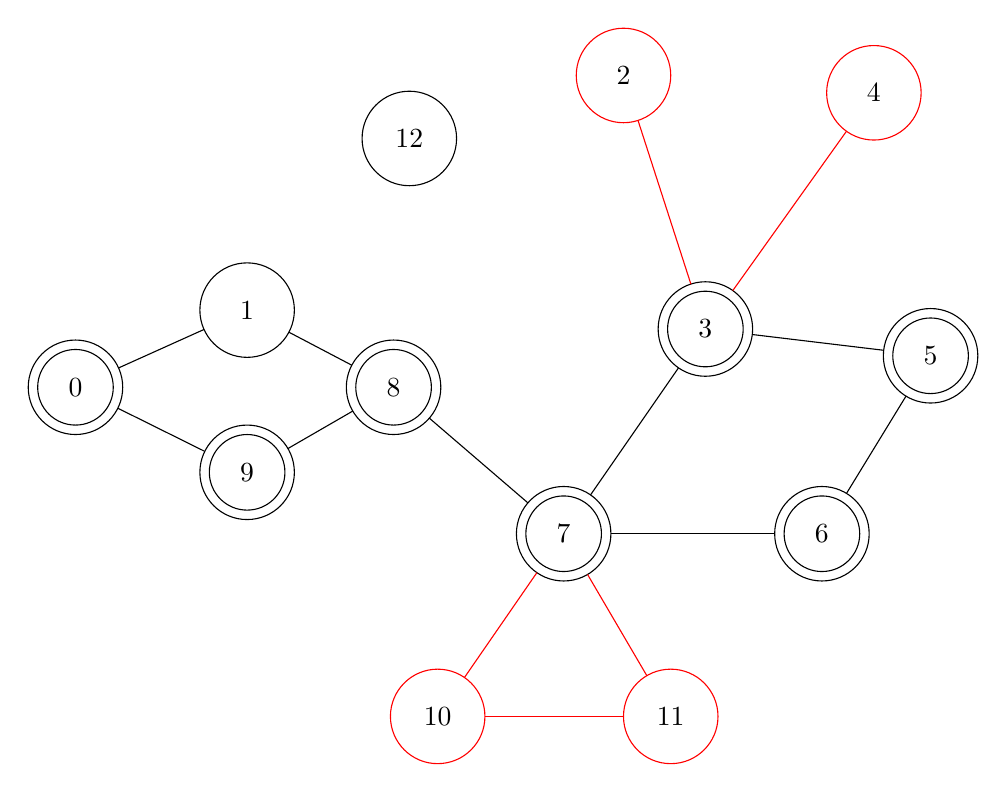
\begin{tikzpicture}[scale=0.2]
    \tikzstyle{every node}+=[inner sep=0pt]
    \draw [black] (5.4,-28.9) circle (3);
    \draw (5.4,-28.9) node {$0$};
    \draw [black] (5.4,-28.9) circle (2.4);
    \draw [black] (16.3,-24) circle (3);
    \draw (16.3,-24) node {$1$};
    \draw [black] (16.3,-34.3) circle (3);
    \draw (16.3,-34.3) node {$9$};
    \draw [black] (16.3,-34.3) circle (2.4);
    \draw [black] (25.6,-28.9) circle (3);
    \draw (25.6,-28.9) node {$8$};
    \draw [black] (25.6,-28.9) circle (2.4);
    \draw [black] (36.4,-38.2) circle (3);
    \draw (36.4,-38.2) node {$7$};
    \draw [black] (36.4,-38.2) circle (2.4);
    \draw [red] (28.4,-49.8) circle (3);
    \draw (28.4,-49.8) node {$10$};
    \draw [red] (43.2,-49.8) circle (3);
    \draw (43.2,-49.8) node {$11$};
    \draw [black] (52.8,-38.2) circle (3);
    \draw (52.8,-38.2) node {$6$};
    \draw [black] (52.8,-38.2) circle (2.4);
    \draw [black] (59.7,-26.9) circle (3);
    \draw (59.7,-26.9) node {$5$};
    \draw [black] (59.7,-26.9) circle (2.4);
    \draw [black] (45.4,-25.2) circle (3);
    \draw (45.4,-25.2) node {$3$};
    \draw [black] (45.4,-25.2) circle (2.4);
    \draw [red] (56.1,-10.2) circle (3);
    \draw (56.1,-10.2) node {$4$};
    \draw [red] (40.2,-9.1) circle (3);
    \draw (40.2,-9.1) node {$2$};
    \draw [black] (26.6,-13.1) circle (3);
    \draw (26.6,-13.1) node {$12$};
    \draw [black] (8.14,-27.67) -- (13.56,-25.23);
    \draw [black] (8.09,-30.23) -- (13.61,-32.97);
    \draw [black] (18.95,-25.4) -- (22.95,-27.5);
    \draw [black] (18.89,-32.79) -- (23.01,-30.41);
    \draw [black] (27.87,-30.86) -- (34.13,-36.24);
    \draw [red] (34.7,-40.67) -- (30.1,-47.33);
    \draw [red] (37.92,-40.79) -- (41.68,-47.21);
    \draw [red] (31.4,-49.8) -- (40.2,-49.8);
    \draw [black] (39.4,-38.2) -- (49.8,-38.2);
    \draw [black] (38.11,-35.73) -- (43.69,-27.67);
    \draw [black] (48.38,-25.55) -- (56.72,-26.55);
    \draw [black] (54.36,-35.64) -- (58.14,-29.46);
    \draw [red] (47.14,-22.76) -- (54.36,-12.64);
    \draw [red] (44.48,-22.35) -- (41.12,-11.95);
    \end{tikzpicture}
\end{center}
\end{figure}

Now we backtrack and we return to the node 8, and we continue doing the DFS 

\begin{figure}[H]
\begin{center}
    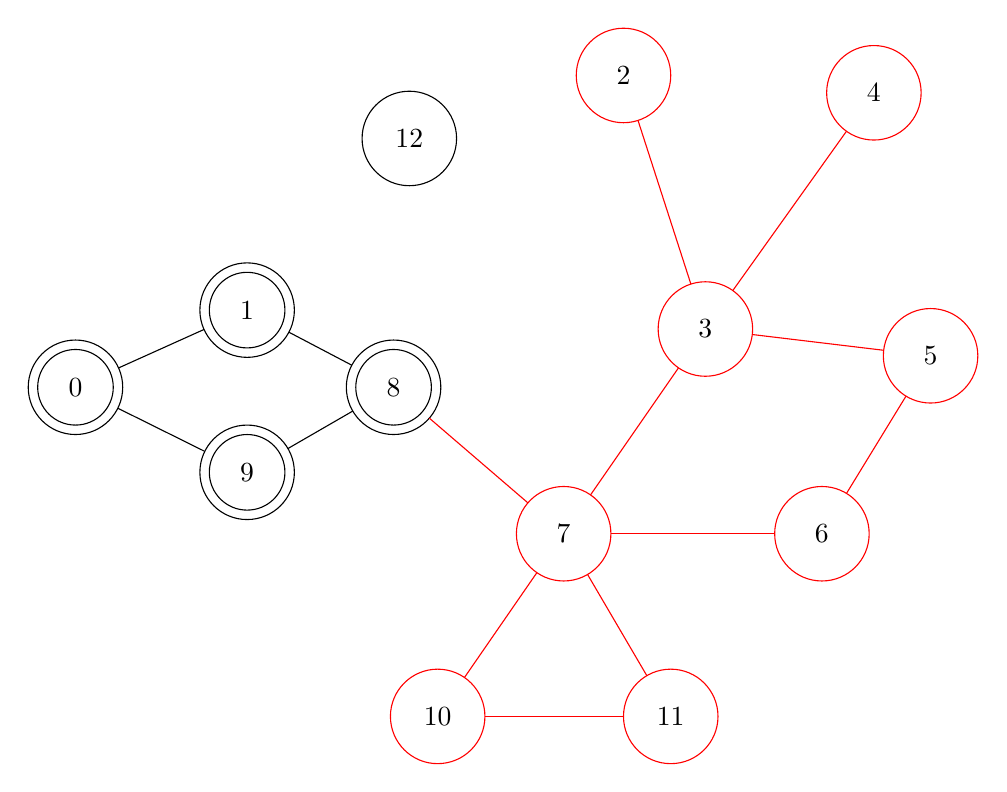
\begin{tikzpicture}[scale=0.2]
    \tikzstyle{every node}+=[inner sep=0pt]
    \draw [black] (5.4,-28.9) circle (3);
    \draw (5.4,-28.9) node {$0$};
    \draw [black] (5.4,-28.9) circle (2.4);
    \draw [black] (16.3,-24) circle (3);
    \draw (16.3,-24) node {$1$};
    \draw [black] (16.3,-24) circle (2.4);
    \draw [black] (16.3,-34.3) circle (3);
    \draw (16.3,-34.3) node {$9$};
    \draw [black] (16.3,-34.3) circle (2.4);
    \draw [black] (25.6,-28.9) circle (3);
    \draw (25.6,-28.9) node {$8$};
    \draw [black] (25.6,-28.9) circle (2.4);
    \draw [red] (36.4,-38.2) circle (3);
    \draw (36.4,-38.2) node {$7$};
    \draw [red] (28.4,-49.8) circle (3);
    \draw (28.4,-49.8) node {$10$};
    \draw [red] (43.2,-49.8) circle (3);
    \draw (43.2,-49.8) node {$11$};
    \draw [red] (52.8,-38.2) circle (3);
    \draw (52.8,-38.2) node {$6$};
    \draw [red] (59.7,-26.9) circle (3);
    \draw (59.7,-26.9) node {$5$};
    \draw [red] (45.4,-25.2) circle (3);
    \draw (45.4,-25.2) node {$3$};
    \draw [red] (56.1,-10.2) circle (3);
    \draw (56.1,-10.2) node {$4$};
    \draw [red] (40.2,-9.1) circle (3);
    \draw (40.2,-9.1) node {$2$};
    \draw [black] (26.6,-13.1) circle (3);
    \draw (26.6,-13.1) node {$12$};
    \draw [black] (8.14,-27.67) -- (13.56,-25.23);
    \draw [black] (8.09,-30.23) -- (13.61,-32.97);
    \draw [black] (18.95,-25.4) -- (22.95,-27.5);
    \draw [black] (18.89,-32.79) -- (23.01,-30.41);
    \draw [red] (27.87,-30.86) -- (34.13,-36.24);
    \draw [red] (34.7,-40.67) -- (30.1,-47.33);
    \draw [red] (37.92,-40.79) -- (41.68,-47.21);
    \draw [red] (31.4,-49.8) -- (40.2,-49.8);
    \draw [red] (39.4,-38.2) -- (49.8,-38.2);
    \draw [red] (38.11,-35.73) -- (43.69,-27.67);
    \draw [red] (48.38,-25.55) -- (56.72,-26.55);
    \draw [red] (54.36,-35.64) -- (58.14,-29.46);
    \draw [red] (47.14,-22.76) -- (54.36,-12.64);
    \draw [red] (44.48,-22.35) -- (41.12,-11.95);
    \end{tikzpicture}
\end{center}
\end{figure}

Again we have a cycle so we bakctrack and we have visited all the nodes

\begin{figure}[H]
\begin{center}
    \begin{tikzpicture}[scale=0.2]
    \tikzstyle{every node}+=[inner sep=0pt]
    \draw [red] (5.4,-28.9) circle (3);
    \draw (5.4,-28.9) node {$0$};
    \draw [red] (16.3,-24) circle (3);
    \draw (16.3,-24) node {$1$};
    \draw [red] (16.3,-34.3) circle (3);
    \draw (16.3,-34.3) node {$9$};
    \draw [red] (25.6,-28.9) circle (3);
    \draw (25.6,-28.9) node {$8$};
    \draw [red] (36.4,-38.2) circle (3);
    \draw (36.4,-38.2) node {$7$};
    \draw [red] (28.4,-49.8) circle (3);
    \draw (28.4,-49.8) node {$10$};
    \draw [red] (43.2,-49.8) circle (3);
    \draw (43.2,-49.8) node {$11$};
    \draw [red] (52.8,-38.2) circle (3);
    \draw (52.8,-38.2) node {$6$};
    \draw [red] (59.7,-26.9) circle (3);
    \draw (59.7,-26.9) node {$5$};
    \draw [red] (45.4,-25.2) circle (3);
    \draw (45.4,-25.2) node {$3$};
    \draw [red] (56.1,-10.2) circle (3);
    \draw (56.1,-10.2) node {$4$};
    \draw [red] (40.2,-9.1) circle (3);
    \draw (40.2,-9.1) node {$2$};
    \draw [black] (26.6,-13.1) circle (3);
    \draw (26.6,-13.1) node {$12$};
    \draw [red] (8.14,-27.67) -- (13.56,-25.23);
    \draw [red] (8.09,-30.23) -- (13.61,-32.97);
    \draw [red] (18.95,-25.4) -- (22.95,-27.5);
    \draw [red] (18.89,-32.79) -- (23.01,-30.41);
    \draw [red] (27.87,-30.86) -- (34.13,-36.24);
    \draw [red] (34.7,-40.67) -- (30.1,-47.33);
    \draw [red] (37.92,-40.79) -- (41.68,-47.21);
    \draw [red] (31.4,-49.8) -- (40.2,-49.8);
    \draw [red] (39.4,-38.2) -- (49.8,-38.2);
    \draw [red] (38.11,-35.73) -- (43.69,-27.67);
    \draw [red] (48.38,-25.55) -- (56.72,-26.55);
    \draw [red] (54.36,-35.64) -- (58.14,-29.46);
    \draw [red] (47.14,-22.76) -- (54.36,-12.64);
    \draw [red] (44.48,-22.35) -- (41.12,-11.95);
    \end{tikzpicture}
\end{center}
\end{figure}

So, how can we made this using some code? I've written some code to explain this clearly

\begin{lstlisting}
    #include <bits/stdc++.h>

    using namespace std;
    
    typedef long long int lli;
    typedef vector< lli > vi;
    
    /* A graph is a set of vertices and edges. Also we need to know that
        we can represent a graph using:
        -> An adjacency matrix G[u][v] = w
        -> An adjacency list u -> (v, w)
        -> An edge list (u, v, w)
        To this implementation I've used an adjacency list
     */
    struct Graph{
    
        /* As I mentioned before I'm using an adjacency list, so each
            node has an adjacency list, and each node has it's value and it's
            visited state
         */
        struct Node{
    
            bool visited;
            lli value;
            vi adjList;
    
            Node(){
                value = 0;
                visited = false;
            }
        };
    
        //Set of nodes
        vector< Node > nodes;
        lli size;
    
        Graph( lli size ){
            this -> size = size;
            nodes.assign( size, Node() );
        }
    
        /* This function connects a node to our graph
        param: (lli)from: the source node
        param: (lli)to: the destination node 
        return: nothing    */
        void connect(lli from, lli to){
            nodes[ from ].adjList.push_back( to );
            nodes[ to ].adjList.push_back( from );
        }
    
        /* This function makes a Depth First Search
        param: (lli)i: the index of the node to search 
        return: nothing    */
        void DFS( lli i ){
            nodes[ i ].visited = true;
            //This line is using to verify if the DFS made is correct
            nodes[ i ].value = 1;
            for(int j = 0; j < nodes[ i ].adjList.size(); j++){
                lli u = nodes[ i ].adjList[ j ];
                if( !nodes[ u ].visited )
                    DFS( u );
            }
        }    
    
        void print(){
            cout << endl;
            for( int i = 0; i < nodes.size(); i++){
                cout << i << " " << nodes[ i ].value << endl;
            }
            cout << endl;
        }
    };
    
    int main(){
    
        lli n_nodes, n_connections, from, to;
        
        cin >> n_nodes >> n_connections;
        Graph graph( n_nodes );
        while(n_connections--){
            cin >> from >> to;
            graph.connect( from, to );
        }
    
        graph.print();
    
        graph.DFS( 0 );
    
        graph.print();
        
        return 0;
    }    
\end{lstlisting}

Just consider that this implementations of the Depth First Search is recusive and in some cases it does not work. 

\subsubsection{Finding components}
An application of the DFS is find components, it is very simple to understand, let's use the next:

\begin{figure}[H]
\begin{center}
    \begin{tikzpicture}[scale=0.2]
    \tikzstyle{every node}+=[inner sep=0pt]
    \draw [black] (4.2,-3.9) circle (3);
    \draw (4.2,-3.9) node {$6$};
    \draw [black] (3.5,-12.6) circle (3);
    \draw (3.5,-12.6) node {$7$};
    \draw [black] (12.4,-8.2) circle (3);
    \draw (12.4,-8.2) node {$11$};
    \draw [black] (26.6,-6.3) circle (3);
    \draw (26.6,-6.3) node {$4$};
    \draw [black] (26.6,-18.9) circle (3);
    \draw (26.6,-18.9) node {$8$};
    \draw [black] (40.5,-6.3) circle (3);
    \draw (40.5,-6.3) node {$0$};
    \draw [black] (43.7,-21.6) circle (3);
    \draw (43.7,-21.6) node {$14$};
    \draw [black] (55.3,-9.6) circle (3);
    \draw (55.3,-9.6) node {$13$};
    \draw [black] (4.4,-31.7) circle (3);
    \draw (4.4,-31.7) node {$12$};
    \draw [black] (21.6,-45) circle (3);
    \draw (21.6,-45) node {$5$};
    \draw [black] (17.6,-35.1) circle (3);
    \draw (17.6,-35.1) node {$1$};
    \draw [black] (11.6,-51) circle (3);
    \draw (11.6,-51) node {$17$};
    \draw [black] (26.6,-53.4) circle (3);
    \draw (26.6,-53.4) node {$16$};
    \draw [black] (55.3,-32.5) circle (3);
    \draw (55.3,-32.5) node {$15$};
    \draw [black] (66.1,-25.3) circle (3);
    \draw (66.1,-25.3) node {$10$};
    \draw [black] (64.5,-44.9) circle (3);
    \draw (64.5,-44.9) node {$2$};
    \draw [black] (48.1,-51.1) circle (3);
    \draw (48.1,-51.1) node {$9$};
    \draw [black] (38.7,-35.1) circle (3);
    \draw (38.7,-35.1) node {$3$};
    \draw [black] (3.96,-6.89) -- (3.74,-9.61);
    \draw [black] (6.19,-11.27) -- (9.71,-9.53);
    \draw [black] (6.86,-5.29) -- (9.74,-6.81);
    \draw [black] (26.6,-9.3) -- (26.6,-15.9);
    \draw [black] (38.28,-8.31) -- (28.82,-16.89);
    \draw [black] (37.5,-6.3) -- (29.6,-6.3);
    \draw [black] (43.43,-6.95) -- (52.37,-8.95);
    \draw [black] (41.11,-9.24) -- (43.09,-18.66);
    \draw [black] (29.56,-19.37) -- (40.74,-21.13);
    \draw [black] (45.79,-19.44) -- (53.21,-11.76);
    \draw [black] (20.48,-42.22) -- (18.72,-37.88);
    \draw [black] (19.03,-46.54) -- (14.17,-49.46);
    \draw [black] (23.13,-47.58) -- (25.07,-50.82);
    \draw [black] (40.22,-37.69) -- (46.58,-48.51);
    \draw [black] (54.22,-35.3) -- (49.18,-48.3);
    \draw [black] (57.09,-34.91) -- (62.71,-42.49);
    \draw [black] (50.91,-50.04) -- (61.69,-45.96);
    \draw [black] (57.8,-30.84) -- (63.6,-26.96);
    \end{tikzpicture}
\end{center}        
\end{figure}

As we can see we have components that are not connected. If we separate in subsets we get:
\begin{itemize}
    \item { $A = { 6, 11, 7 }$ }
    \item { $B = { 4, 0, 13, 14, 8 }$ }
    \item { $C = { 12 }$ }
    \item { $D = { 1, 5, 16, 17 }$ }
    \item { $E = { 3, 9, 2, 15, 10 }$ }
\end{itemize}

Each subset we go to call it as component. Now we know what is a component but we do not know how to identify each component yet. To solve this problem we can use the Depth First Search. Maybe you noticed that if the graph have a node that is not connected the DFS never verify that node, so we can made n DFS, one for each component if and just if the current node has not been visited.
So, if we code this we need just modify the next:\\\\

Modify the struct \textbf{Node}, we need to add the attribute component, something like this:
\begin{lstlisting}
    struct Node{
        lli value;
        bool visited;
        lli component;
        vector< lli > adjList;
        Node(){
            value = 0;
            visited = false;
            component = 0;
        }        
    };
\end{lstlisting}

Then we need to modify our DFS function, because we go to assign something to the component attribute:

\begin{lstlisting}
    void DFS( lli i, lli count ){
        nodes[ i ].visited = true;
        nodes[ i ].value = 1;
        nodes[ i ].component = count;
        for( int j = 0; j < nodes[ i ].adjList.size(); j++ ){
            lli u = nodes[ i ].adjList[ j ];
            if( !nodes[ u ].visited )
                DFS( u, count );
        }
    }
\end{lstlisting}

And finally we need to write the code to the fundComponents function. Here we need to made n callings to the DFS function, many as we need, and we go to made the DFS if and just if the current node has not been visited yet.

\begin{lstlisting}
    lli findComponents(){
        lli count = 0;
        for( int i = 0; i < size; i++ )
            if( !nodes[ i ].visited )
                DFS( i, count++ );
        return count;
    }
\end{lstlisting}